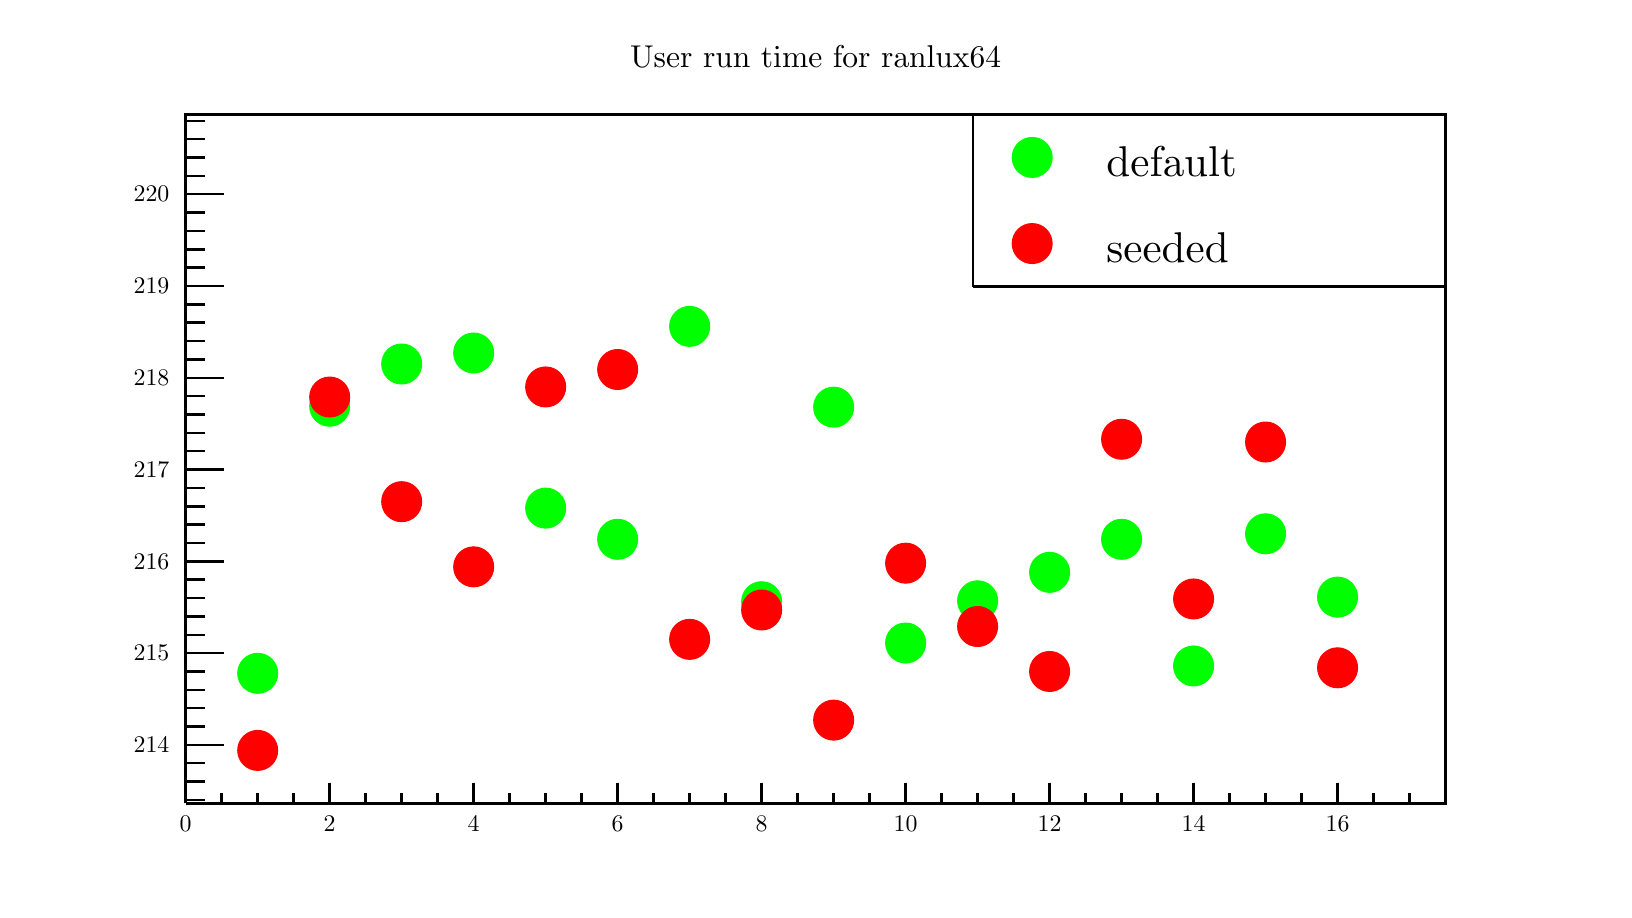
\begin{tikzpicture}
\pgfdeclareplotmark{cross} {
\pgfpathmoveto{\pgfpoint{-0.3\pgfplotmarksize}{\pgfplotmarksize}}
\pgfpathlineto{\pgfpoint{+0.3\pgfplotmarksize}{\pgfplotmarksize}}
\pgfpathlineto{\pgfpoint{+0.3\pgfplotmarksize}{0.3\pgfplotmarksize}}
\pgfpathlineto{\pgfpoint{+1\pgfplotmarksize}{0.3\pgfplotmarksize}}
\pgfpathlineto{\pgfpoint{+1\pgfplotmarksize}{-0.3\pgfplotmarksize}}
\pgfpathlineto{\pgfpoint{+0.3\pgfplotmarksize}{-0.3\pgfplotmarksize}}
\pgfpathlineto{\pgfpoint{+0.3\pgfplotmarksize}{-1.\pgfplotmarksize}}
\pgfpathlineto{\pgfpoint{-0.3\pgfplotmarksize}{-1.\pgfplotmarksize}}
\pgfpathlineto{\pgfpoint{-0.3\pgfplotmarksize}{-0.3\pgfplotmarksize}}
\pgfpathlineto{\pgfpoint{-1.\pgfplotmarksize}{-0.3\pgfplotmarksize}}
\pgfpathlineto{\pgfpoint{-1.\pgfplotmarksize}{0.3\pgfplotmarksize}}
\pgfpathlineto{\pgfpoint{-0.3\pgfplotmarksize}{0.3\pgfplotmarksize}}
\pgfpathclose
\pgfusepathqstroke
}
\pgfdeclareplotmark{cross*} {
\pgfpathmoveto{\pgfpoint{-0.3\pgfplotmarksize}{\pgfplotmarksize}}
\pgfpathlineto{\pgfpoint{+0.3\pgfplotmarksize}{\pgfplotmarksize}}
\pgfpathlineto{\pgfpoint{+0.3\pgfplotmarksize}{0.3\pgfplotmarksize}}
\pgfpathlineto{\pgfpoint{+1\pgfplotmarksize}{0.3\pgfplotmarksize}}
\pgfpathlineto{\pgfpoint{+1\pgfplotmarksize}{-0.3\pgfplotmarksize}}
\pgfpathlineto{\pgfpoint{+0.3\pgfplotmarksize}{-0.3\pgfplotmarksize}}
\pgfpathlineto{\pgfpoint{+0.3\pgfplotmarksize}{-1.\pgfplotmarksize}}
\pgfpathlineto{\pgfpoint{-0.3\pgfplotmarksize}{-1.\pgfplotmarksize}}
\pgfpathlineto{\pgfpoint{-0.3\pgfplotmarksize}{-0.3\pgfplotmarksize}}
\pgfpathlineto{\pgfpoint{-1.\pgfplotmarksize}{-0.3\pgfplotmarksize}}
\pgfpathlineto{\pgfpoint{-1.\pgfplotmarksize}{0.3\pgfplotmarksize}}
\pgfpathlineto{\pgfpoint{-0.3\pgfplotmarksize}{0.3\pgfplotmarksize}}
\pgfpathclose
\pgfusepathqfillstroke
}
\pgfdeclareplotmark{newstar} {
\pgfpathmoveto{\pgfqpoint{0pt}{\pgfplotmarksize}}
\pgfpathlineto{\pgfqpointpolar{44}{0.5\pgfplotmarksize}}
\pgfpathlineto{\pgfqpointpolar{18}{\pgfplotmarksize}}
\pgfpathlineto{\pgfqpointpolar{-20}{0.5\pgfplotmarksize}}
\pgfpathlineto{\pgfqpointpolar{-54}{\pgfplotmarksize}}
\pgfpathlineto{\pgfqpointpolar{-90}{0.5\pgfplotmarksize}}
\pgfpathlineto{\pgfqpointpolar{234}{\pgfplotmarksize}}
\pgfpathlineto{\pgfqpointpolar{198}{0.5\pgfplotmarksize}}
\pgfpathlineto{\pgfqpointpolar{162}{\pgfplotmarksize}}
\pgfpathlineto{\pgfqpointpolar{134}{0.5\pgfplotmarksize}}
\pgfpathclose
\pgfusepathqstroke
}
\pgfdeclareplotmark{newstar*} {
\pgfpathmoveto{\pgfqpoint{0pt}{\pgfplotmarksize}}
\pgfpathlineto{\pgfqpointpolar{44}{0.5\pgfplotmarksize}}
\pgfpathlineto{\pgfqpointpolar{18}{\pgfplotmarksize}}
\pgfpathlineto{\pgfqpointpolar{-20}{0.5\pgfplotmarksize}}
\pgfpathlineto{\pgfqpointpolar{-54}{\pgfplotmarksize}}
\pgfpathlineto{\pgfqpointpolar{-90}{0.5\pgfplotmarksize}}
\pgfpathlineto{\pgfqpointpolar{234}{\pgfplotmarksize}}
\pgfpathlineto{\pgfqpointpolar{198}{0.5\pgfplotmarksize}}
\pgfpathlineto{\pgfqpointpolar{162}{\pgfplotmarksize}}
\pgfpathlineto{\pgfqpointpolar{134}{0.5\pgfplotmarksize}}
\pgfpathclose
\pgfusepathqfillstroke
}
\definecolor{c}{rgb}{1,1,1};
\draw [color=c, fill=c] (0,0) rectangle (20,10.9387);
\draw [color=c, fill=c] (2,1.09387) rectangle (18,9.84481);
\definecolor{c}{rgb}{0,0,0};
\draw [c,line width=0.9] (2,1.09387) -- (2,9.84481) -- (18,9.84481) -- (18,1.09387) -- (2,1.09387);
\definecolor{c}{rgb}{1,1,1};
\draw [color=c, fill=c] (2,1.09387) rectangle (18,9.84481);
\definecolor{c}{rgb}{0,0,0};
\draw [c,line width=0.9] (2,1.09387) -- (2,9.84481) -- (18,9.84481) -- (18,1.09387) -- (2,1.09387);
\draw [c,line width=0.9] (2,1.09387) -- (18,1.09387);
\draw [c,line width=0.9] (2,1.3564) -- (2,1.09387);
\draw [c,line width=0.9] (2.45714,1.22513) -- (2.45714,1.09387);
\draw [c,line width=0.9] (2.91429,1.22513) -- (2.91429,1.09387);
\draw [c,line width=0.9] (3.37143,1.22513) -- (3.37143,1.09387);
\draw [c,line width=0.9] (3.82857,1.3564) -- (3.82857,1.09387);
\draw [c,line width=0.9] (4.28571,1.22513) -- (4.28571,1.09387);
\draw [c,line width=0.9] (4.74286,1.22513) -- (4.74286,1.09387);
\draw [c,line width=0.9] (5.2,1.22513) -- (5.2,1.09387);
\draw [c,line width=0.9] (5.65714,1.3564) -- (5.65714,1.09387);
\draw [c,line width=0.9] (6.11429,1.22513) -- (6.11429,1.09387);
\draw [c,line width=0.9] (6.57143,1.22513) -- (6.57143,1.09387);
\draw [c,line width=0.9] (7.02857,1.22513) -- (7.02857,1.09387);
\draw [c,line width=0.9] (7.48571,1.3564) -- (7.48571,1.09387);
\draw [c,line width=0.9] (7.94286,1.22513) -- (7.94286,1.09387);
\draw [c,line width=0.9] (8.4,1.22513) -- (8.4,1.09387);
\draw [c,line width=0.9] (8.85714,1.22513) -- (8.85714,1.09387);
\draw [c,line width=0.9] (9.31429,1.3564) -- (9.31429,1.09387);
\draw [c,line width=0.9] (9.77143,1.22513) -- (9.77143,1.09387);
\draw [c,line width=0.9] (10.2286,1.22513) -- (10.2286,1.09387);
\draw [c,line width=0.9] (10.6857,1.22513) -- (10.6857,1.09387);
\draw [c,line width=0.9] (11.1429,1.3564) -- (11.1429,1.09387);
\draw [c,line width=0.9] (11.6,1.22513) -- (11.6,1.09387);
\draw [c,line width=0.9] (12.0571,1.22513) -- (12.0571,1.09387);
\draw [c,line width=0.9] (12.5143,1.22513) -- (12.5143,1.09387);
\draw [c,line width=0.9] (12.9714,1.3564) -- (12.9714,1.09387);
\draw [c,line width=0.9] (13.4286,1.22513) -- (13.4286,1.09387);
\draw [c,line width=0.9] (13.8857,1.22513) -- (13.8857,1.09387);
\draw [c,line width=0.9] (14.3429,1.22513) -- (14.3429,1.09387);
\draw [c,line width=0.9] (14.8,1.3564) -- (14.8,1.09387);
\draw [c,line width=0.9] (15.2571,1.22513) -- (15.2571,1.09387);
\draw [c,line width=0.9] (15.7143,1.22513) -- (15.7143,1.09387);
\draw [c,line width=0.9] (16.1714,1.22513) -- (16.1714,1.09387);
\draw [c,line width=0.9] (16.6286,1.3564) -- (16.6286,1.09387);
\draw [c,line width=0.9] (16.6286,1.3564) -- (16.6286,1.09387);
\draw [c,line width=0.9] (17.0857,1.22513) -- (17.0857,1.09387);
\draw [c,line width=0.9] (17.5429,1.22513) -- (17.5429,1.09387);
\draw [c,line width=0.9] (18,1.22513) -- (18,1.09387);
\draw [anchor=base] (2,0.732891) node[scale=0.861703, color=c, rotate=0]{0};
\draw [anchor=base] (3.82857,0.732891) node[scale=0.861703, color=c, rotate=0]{2};
\draw [anchor=base] (5.65714,0.732891) node[scale=0.861703, color=c, rotate=0]{4};
\draw [anchor=base] (7.48571,0.732891) node[scale=0.861703, color=c, rotate=0]{6};
\draw [anchor=base] (9.31429,0.732891) node[scale=0.861703, color=c, rotate=0]{8};
\draw [anchor=base] (11.1429,0.732891) node[scale=0.861703, color=c, rotate=0]{10};
\draw [anchor=base] (12.9714,0.732891) node[scale=0.861703, color=c, rotate=0]{12};
\draw [anchor=base] (14.8,0.732891) node[scale=0.861703, color=c, rotate=0]{14};
\draw [anchor=base] (16.6286,0.732891) node[scale=0.861703, color=c, rotate=0]{16};
\draw [c,line width=0.9] (2,1.09387) -- (2,9.84481);
\draw [c,line width=0.9] (2.48,1.83695) -- (2,1.83695);
\draw [c,line width=0.9] (2.24,2.07008) -- (2,2.07008);
\draw [c,line width=0.9] (2.24,2.3032) -- (2,2.3032);
\draw [c,line width=0.9] (2.24,2.53633) -- (2,2.53633);
\draw [c,line width=0.9] (2.24,2.76945) -- (2,2.76945);
\draw [c,line width=0.9] (2.48,3.00258) -- (2,3.00258);
\draw [c,line width=0.9] (2.24,3.23571) -- (2,3.23571);
\draw [c,line width=0.9] (2.24,3.46883) -- (2,3.46883);
\draw [c,line width=0.9] (2.24,3.70196) -- (2,3.70196);
\draw [c,line width=0.9] (2.24,3.93508) -- (2,3.93508);
\draw [c,line width=0.9] (2.48,4.16821) -- (2,4.16821);
\draw [c,line width=0.9] (2.24,4.40133) -- (2,4.40133);
\draw [c,line width=0.9] (2.24,4.63446) -- (2,4.63446);
\draw [c,line width=0.9] (2.24,4.86758) -- (2,4.86758);
\draw [c,line width=0.9] (2.24,5.10071) -- (2,5.10071);
\draw [c,line width=0.9] (2.48,5.33383) -- (2,5.33383);
\draw [c,line width=0.9] (2.24,5.56696) -- (2,5.56696);
\draw [c,line width=0.9] (2.24,5.80008) -- (2,5.80008);
\draw [c,line width=0.9] (2.24,6.03321) -- (2,6.03321);
\draw [c,line width=0.9] (2.24,6.26633) -- (2,6.26633);
\draw [c,line width=0.9] (2.48,6.49946) -- (2,6.49946);
\draw [c,line width=0.9] (2.24,6.73258) -- (2,6.73258);
\draw [c,line width=0.9] (2.24,6.96571) -- (2,6.96571);
\draw [c,line width=0.9] (2.24,7.19883) -- (2,7.19883);
\draw [c,line width=0.9] (2.24,7.43196) -- (2,7.43196);
\draw [c,line width=0.9] (2.48,7.66508) -- (2,7.66508);
\draw [c,line width=0.9] (2.24,7.89821) -- (2,7.89821);
\draw [c,line width=0.9] (2.24,8.13134) -- (2,8.13134);
\draw [c,line width=0.9] (2.24,8.36446) -- (2,8.36446);
\draw [c,line width=0.9] (2.24,8.59759) -- (2,8.59759);
\draw [c,line width=0.9] (2.48,8.83071) -- (2,8.83071);
\draw [c,line width=0.9] (2.48,1.83695) -- (2,1.83695);
\draw [c,line width=0.9] (2.24,1.60383) -- (2,1.60383);
\draw [c,line width=0.9] (2.24,1.3707) -- (2,1.3707);
\draw [c,line width=0.9] (2.24,1.13758) -- (2,1.13758);
\draw [c,line width=0.9] (2.48,8.83071) -- (2,8.83071);
\draw [c,line width=0.9] (2.24,9.06384) -- (2,9.06384);
\draw [c,line width=0.9] (2.24,9.29696) -- (2,9.29696);
\draw [c,line width=0.9] (2.24,9.53009) -- (2,9.53009);
\draw [c,line width=0.9] (2.24,9.76321) -- (2,9.76321);
\draw [anchor= east] (1.9,1.83695) node[scale=0.861703, color=c, rotate=0]{214};
\draw [anchor= east] (1.9,3.00258) node[scale=0.861703, color=c, rotate=0]{215};
\draw [anchor= east] (1.9,4.16821) node[scale=0.861703, color=c, rotate=0]{216};
\draw [anchor= east] (1.9,5.33383) node[scale=0.861703, color=c, rotate=0]{217};
\draw [anchor= east] (1.9,6.49946) node[scale=0.861703, color=c, rotate=0]{218};
\draw [anchor= east] (1.9,7.66508) node[scale=0.861703, color=c, rotate=0]{219};
\draw [anchor= east] (1.9,8.83071) node[scale=0.861703, color=c, rotate=0]{220};
\definecolor{c}{rgb}{0,1,0};
\foreach \P in {(2.91429,2.74614), (3.82857,6.13811), (4.74286,6.6743), (5.65714,6.81418), (6.57143,4.84427), (7.48571,4.44796), (8.4,7.15221), (9.31429,3.65533), (10.2286,6.12646), (11.1429,3.1308), (12.0571,3.66699), (12.9714,4.02833),
 (13.8857,4.44796), (14.8,2.83939), (15.7143,4.51789), (16.6286,3.71361)}{\draw[mark options={color=c,fill=c},mark size=7.207207pt,mark=*] plot coordinates {\P};}
\definecolor{c}{rgb}{1,0,0};
\foreach \P in {(2.91429,1.76702), (3.82857,6.25468), (4.74286,4.92586), (5.65714,4.09827), (6.57143,6.3829), (7.48571,6.60436), (8.4,3.17742), (9.31429,3.55042), (10.2286,2.15167), (11.1429,4.14489), (12.0571,3.34061), (12.9714,2.76945),
 (13.8857,5.71849), (14.8,3.6903), (15.7143,5.68352), (16.6286,2.81608)}{\draw[mark options={color=c,fill=c},mark size=7.207207pt,mark=*] plot coordinates {\P};}
\definecolor{c}{rgb}{1,1,1};
\draw [color=c, fill=c] (12,7.65707) rectangle (18,9.84481);
\definecolor{c}{rgb}{0,0,0};
\draw [c,line width=0.9] (12,7.65707) -- (18,7.65707);
\draw [c,line width=0.9] (18,7.65707) -- (18,9.84481);
\draw [c,line width=0.9] (18,9.84481) -- (12,9.84481);
\draw [c,line width=0.9] (12,9.84481) -- (12,7.65707);
\draw [anchor=base west] (13.5,9.05175) node[scale=1.55662, color=c, rotate=0]{default};
\definecolor{c}{rgb}{1,1,1};
\draw [c] (12.225,8.91502) -- (13.275,8.91502) -- (13.275,9.68073) -- (12.225,9.68073);
\draw [c,line width=0.9] (12.225,9.29787) -- (13.275,9.29787);
\definecolor{c}{rgb}{0,1,0};
\foreach \P in {(12.75,9.29787)}{\draw[mark options={color=c,fill=c},mark size=7.207207pt,mark=*] plot coordinates {\P};}
\definecolor{c}{rgb}{0,0,0};
\draw [anchor=base west] (13.5,7.95788) node[scale=1.55662, color=c, rotate=0]{seeded};
\definecolor{c}{rgb}{1,1,1};
\draw [c] (12.225,7.82115) -- (13.275,7.82115) -- (13.275,8.58686) -- (12.225,8.58686);
\draw [c,line width=0.9] (12.225,8.204) -- (13.275,8.204);
\definecolor{c}{rgb}{1,0,0};
\foreach \P in {(12.75,8.204)}{\draw[mark options={color=c,fill=c},mark size=7.207207pt,mark=*] plot coordinates {\P};}
\definecolor{c}{rgb}{0,0,0};
\draw (10,10.5832) node[scale=1.13967, color=c, rotate=0]{User run time for ranlux64};
\end{tikzpicture}
